% !TeX root = ../../main.tex
\section{Experiments}\label{section:experiments}

Three experiments were implemented to demonstrate how the smartphone can help with common interactions when using \gls{VR} software.
To achieve consistency amongst all experiments in terms of optics and basic functionality, a parent class was implemented. The parent class implements utilities, which are required and inherited by each experiment. It also sets up a basic scene, which contains a background, a floor, and lights. Additionally, it handles the connection to the \gls{UBII} Server.

Some three-dimensional models, used in the following experiments, were downloaded from the internet. Those resources are listed in Appendix~\ref{chapter:external-assets-used} including their licenses.


\subsection{Model Viewer}\label{subsection:model-viewer}

\acrlong{VR} offers a new way of experiencing three-dimensional content. It is convenient to view a model from different angles and gives a feel of a real presence of the object. Applications where the user can load custom three-dimensional models into the scene and use the app to explorer the models are commonly called \enquote{model viewers}. One instance of such a model viewer is the online model viewing platform Sketchfab\footnote{Sketchfab is an online platform where one can publish and view three-dimensional content. Website: \href{https://sketchfab.com}{www.sketchfab.com}} which supports Web\gls{VR} since 2016, to view three-dimensional models online.~\cite{Denoyel.2016}. 

Especially model viewing applications can be enhanced with a smartphone. Without the need for changing the position of the \gls{HMD} or using an expensive hand motion tracking system, the orientation of the models can be manipulated.
\citeauthor{Katzakis.2010} implemented such a system without using \gls{VR}. Their approach uses a smartphone to rotate a model which is displayed on a conventional display. They use a similar setup as the one presented in this thesis, in which the phone is wirelessly connected to a computer where the model is rendered. The orientation data is provided by the magnetometer and, once calibrated to the screen position, is directly mapped to the model~\cite[139]{Katzakis.2010}. In the evaluation of their system, a mouse, a touch pen, and the smartphone were compared. The latter wins in terms of the time it takes to rotate the model to a certain pose~\cite[140]{Katzakis.2010}.
Since this approach turned out to be very successful, it was used in this experiment as well.

To feature how easy it is to view a more complex model using \gls{VR} and the smartphone as a manipulator, a human skeleton model is used. This experiment is the only one supporting more than one smartphone client at the same time, which opens the possibility to implement multi-user scenarios. For every client that connects, a new skeleton model is created. The position is fixed and arranged around the position of the \gls{VR} headset. A scene with multiple connected clients is shown in Figure~\ref{fig:screenshot-exp-mv}.

\begin{figure}[H]
	\centering
	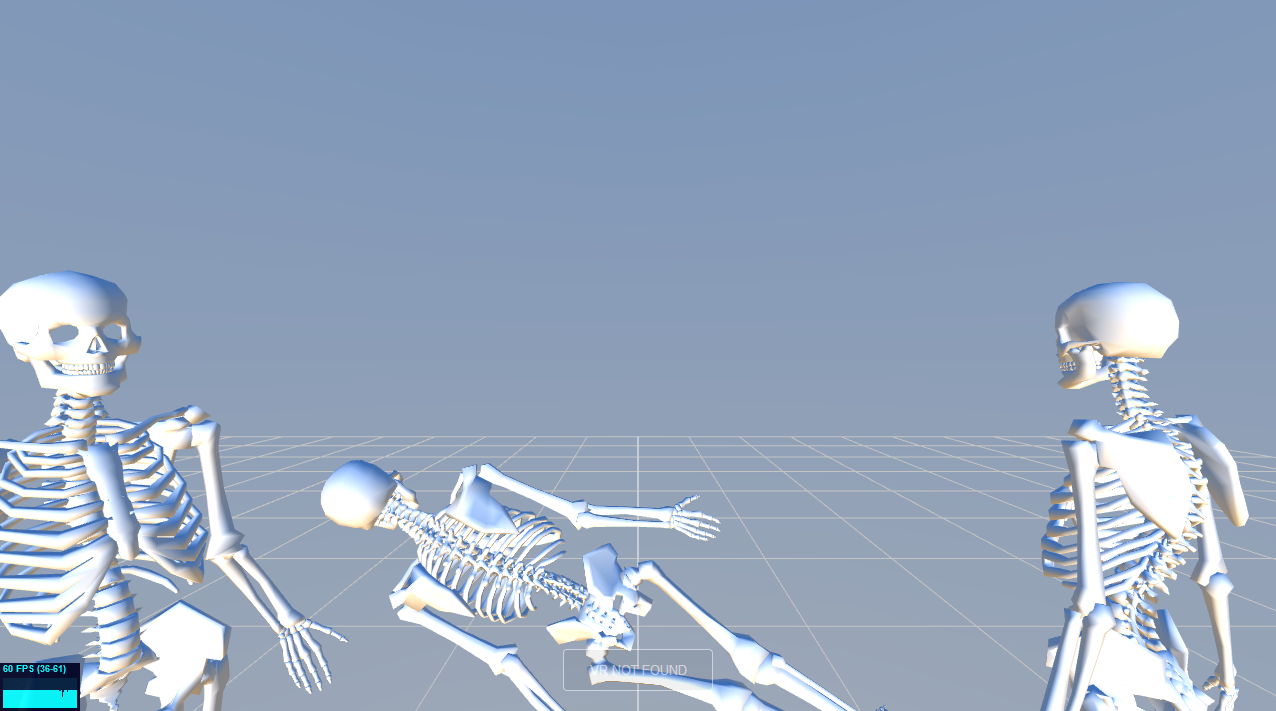
\includegraphics[width=12cm]{figures/implementation/screenshot_exp_mv.png}
	\caption[Screenshot of the model viewer]{A screenshot showing three models, whose rotation is being controlled by three smartphones.}\label{fig:screenshot-exp-mv}
\end{figure}

The experiment always listens for new clients. As soon as one connects, a new Interaction is published, and the resulting Topic subscribed. Since the smart device (see Section~\ref{section:smart-device}) publishes the orientation data in a different format than ThreeJS needs for rendering, a reusable Interaction was created. This Interaction converts the angles from radian to degrees, changes the coordinate system, and publishes them to the \lstinline[breaklines=false]{[client id]/SAVRLaserPointer/orientation} topic. The code for the Interaction is shown in Figure~\ref{fig:ubii-interaction-angles}.

\begin{figure}[H]
	\begin{lstlisting}[language=JavaScript]
  function (input, output, state) {
    if (!input) {
      return;
    }

    const deg2Rad = function(v) {
      return v * Math.PI / 180;
    };

    output.orientation = {
      x: deg2Rad(input.orientation.y),
      y: deg2Rad(input.orientation.x),
      z: deg2Rad(-input.orientation.z)
    };
  }
 \end{lstlisting}
	\caption[A UBII Interaction of model viewer]{This \gls{UBII} Interaction is used to convert the orientation data sent by the smart device to the format ThreeJS needs for rendering. The values are converted by multiplying with an approximate of the number $\Pi$ (\enquote{PI}) and dividing by $180$.}\label{fig:ubii-interaction-angles} %chktex 46
\end{figure}

As in Section~\ref{subsection:topic-data} described, the current implementation does not provide the full angular data needed. This means that the model cannot be rotated upside down, which is very impractical for a model viewing application. However, this can be fixed and is not critical for a proof-of-concept.


\subsection{Laser Pointer}\label{subsection:laser-pointer}

Selecting elements in a virtual world is an essential interaction most \gls{VR} applications use. The selection of elements in a two-dimensional environment with standard input devices like a mouse or touch screen is rather trivial. However, the selection of elements in a three-dimensional environment is problematic because the element might be too far away from the user or the cursor.

Ray casting\footnote{Ray casting describes a technique to determine the objects which intersect with a ray, cast from a given point into a given direction.} is used to solve this problem: A ray, with the virtual device's position as origin, is created. Then, the element first hit by the ray is selected. Implementations without a tracked device, often use the position and orientation of the \gls{HMD}. The ray is fixed to the head of the user and cast along his viewing direction~\cite[23]{Kamm.2018}. This forces the user to keep the head still and look at a particular object to select it until a button is pressed or a specific time has passed.

% maybe explain some more strategies, like in the keyboard chapter
A better solution is the use of handheld controllers, where the position of the controller is used as origin for the ray. This approach is more suited for the laser pointer application because it feels more comfortable to use our natural pointing devices, the hands, for aiming. The positional tracking enables to represent the hand of a user as well as the laser pointer in \gls{VR} at the real-world location. Since a smartphone does not have positional tracking, only the rotation can be synchronized with the one from the real world. However, the virtual laser pointer still needs a position/origin.

%\citeauthor{Argelaguet.2013} evaluated more than 30 different selection techniques for virtual environments, but no technique uses the orientation but not the position of the pointing device~\cite[Table 1]{Argelaguet.2013}.
The user's head position could be used as origin while the smartphone provides the rotation data. Without any smartphone representation in the \gls{VE}, the user would have no visual clue, other than the virtual laser beam, of the rotation of the phone. This becomes a problem when the user's head rotation is unequal to the laser direction because the user cannot see the virtual laser beam. To give the user a better feel for the direction he is pointing at, a visual representation of the smartphone is needed.

As a workaround, to the missing positional data of the device, the approach by \citeauthor{Pietroszek.2014} is used: The ray origin/virtual smartphone position is set to a fixed location relative to the user's head~\cite[Figure 3]{Pietroszek.2014}. The location should be where the phone could be in the real world.

The ray origin is represented by a three-dimensional phone model, whose orientation is synchronized with the one from the last connected smart device client (see Section~\ref{section:smart-device}), similar to the first experiment (see Section~\ref{subsection:model-viewer}). To keep the virtual phone inside the field of view of the user, it rotates relative to the user on the up-axis and moves only on the right/forward-axis.
A line is attached to the front of the phone (the \enquote{laser}) to indicate the direction of the ray, as can be seen in the screenshot of this setup in Figure~\ref{fig:screenshot-exp-lp}.

\begin{figure}[H]
	\centering
	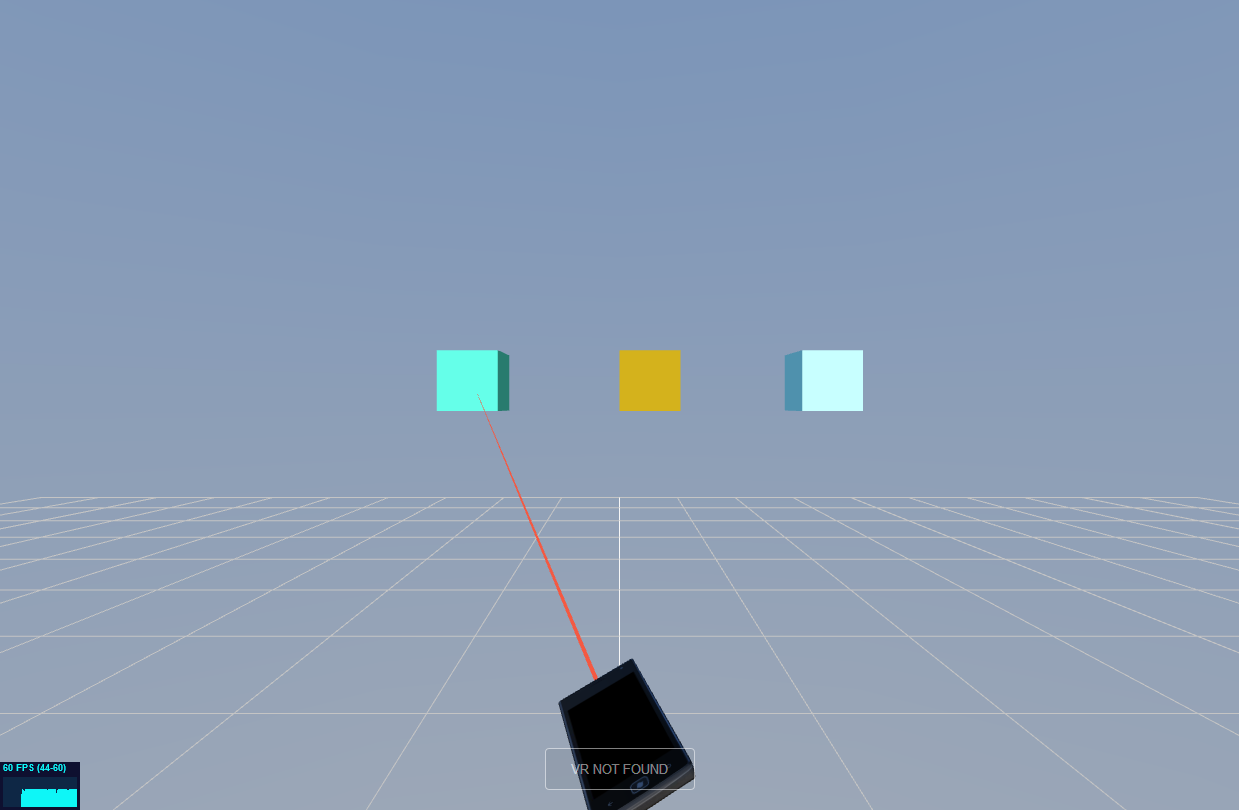
\includegraphics[width=12cm]{figures/implementation/screenshot_exp_lp.png}
	\caption[Screenshot of the laser pointer]{A screenshot, showing the virtual phone, the virtual laser pointer and selectable cubes.}\label{fig:screenshot-exp-lp}
\end{figure}

In addition to the orientation Topic, this implementation subscribes to the \lstinline{TouchEvent} Topic, presented in Chapter~\ref{subsection:ubii-device-definition}. The \lstinline{touch down} event is needed to trigger the actual selection when the user touches the touch display.

To illustrate a selection task with this system, selectable cubes float in front of the user. 
When a randomly colored cube is selected, it will change its color again. This works not only with cubes but with any mesh. Also, the system can trigger any kind of event or action.


\subsection{Virtual Keyboard}\label{subsection:virtual-keyboard}

Text input is not an easy task to perform in \gls{VR}. This is why many applications try to avoid it. However, it is often required for labeling, annotation, entering filenames for saving operations, and setting parameters in visualizations and other productive \gls{VR} software~\cite[2154]{Rhoton.2002}. 

Tilt Brush\footnote{Tilt Brush by Google is a tool for three-dimensional painting in VR. Website: \href{https://www.tiltbrush.com/}{www.tiltbrush.com}} avoids this during the select and load process of scenes, by identifying the scenes with a screenshot of the scene rather than a filename. To save a scene, the user gets a virtual camera attached to his hand motion controller, which he then uses to create a thumbnail of the current scene~\cite{GoogleLLC.2019}. % chktex 13

Some applications use a laser pointer either attached to the motion controller or to the \gls{HMD} to select virtual keys on a two-dimensional image of a keyboard~\cite{WeelcoInc.2017}. A more recent approach is the frequently called \enquote{drum keyboard}, which attaches drum sticks to the hand controllers which are then used to hit three-dimensional keys~\cite{Weisel.2017}.

Other approaches use hand gloves~\cite{Evans.1999,Rhoton.2002}, a real keyboard~\cite{McGill.2015,Walker.2017} or other peripherals~\cite[111\psq]{Gonzalez.2009}. Also, methods like speech recognition~\cite[2154\psqq]{Rhoton.2002} and handwritten character recognition~\cite[113]{Gonzalez.2009} are possible.

Similar to the approach by~\citeauthor{Dias.2018}, who implemented user interfaces using a real smartphone and a virtual representation in the \gls{VE}~\cite[5]{Dias.2018}, this experiment uses a virtual keyboard as seen in Figure~\ref{fig:screenshot-exp-vk}.
The surface of the virtual keyboard is mapped to the touchscreen of the smart device (see Section~\ref{section:smart-device}). The cursor, represented by a blue circle, visualizes the position of the finger on the touchscreen.

\begin{figure}[H]
	\centering
	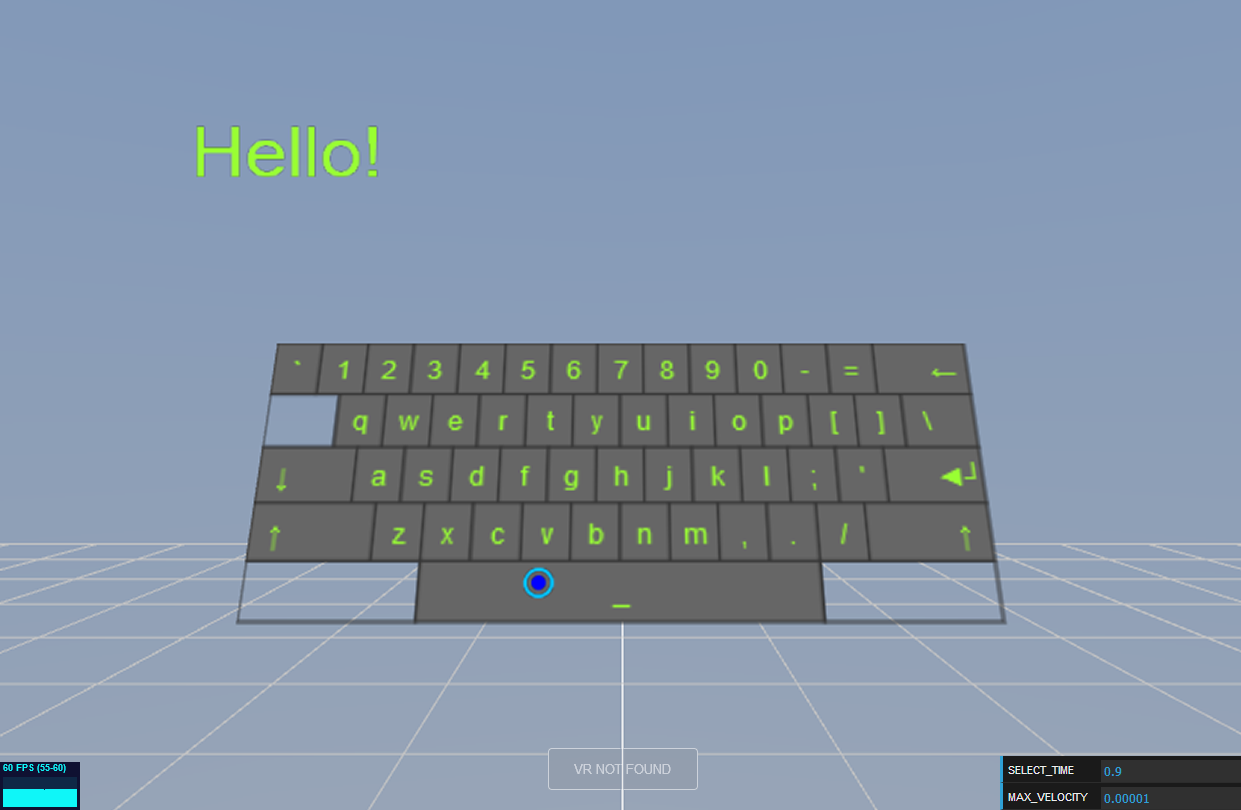
\includegraphics[width=12cm]{figures/implementation/screenshot_exp_vk.png}
	\caption[Screenshot of the virtual keyboard]{This screenshot is showing the virtual keyboard with the blue cursor. The previously typed text is displayed above.}\label{fig:screenshot-exp-vk}
\end{figure}

When executing the keypress on the first touch and without a cursor (like on a regular smartphone keyboard), the user would not know which key he is going to hit with his finger, because his sight is physically obscured by the \gls{HMD}. \citeauthor{Dias.2018} work around this problem by using a Leap Motion sensor, which tracks the whole hand, (see Chapter~\ref{section:motivation}) to visualize the finger positions~\cite[4]{Dias.2018}.

In this implementation, the cursor is only visible when the user is touching the screen. To select a key, the user has to move the cursor on top of a key and then keep the finger there for roughly a second. As long as the user is holding his finger on a key to select it, the blue circle increases in size to display the selection progress.

Three components were implemented as \acrlong{JS} classes for this experiment. The \lstinline{SmartphoneCursor} component uses the touch events and position data to display a blue circle (the cursor) on a given area in the scene. If the touch screen is touched, the position of the circle is synchronized with the position of the finger on the touch screen.

To detect intentional movements, the current position is subtracted by the position of the previous frame. If the length of the resulting vector is smaller than a specific threshold value, it is assumed that the movement was not intentional.

As long as intentional movements are not detected, a timer counts up to a specific value (with the default settings, roughly one second). To visualize the selection progress, the cursor is filled with blue color. After reaching the value, a select event containing the cursor position is sent to the main program and the blue color is removed. 

The second component renders a virtual QWERTY\footnote{The name QWERTY describes the US layout for computer keyboards.} keyboard to the scene. The keyboard layout, whose definition is shown in Figure~\ref{fig:virtual-keyboard-layout}, can be easily adjusted. Every key has a character or an action assigned as well as properties which influence the look. Special keys like the caps, caps lock, enter and delete key are fully functional as known from a real keyboard. When caps lock is activated, the key is drawn in blue, and all characters are display in upper case.

\begin{figure}[H]
	\begin{lstlisting}[language=JavaScript]
  // rows
  [
    // columns
    %\dots%
    [ 
      // keys
      %\dots%
      {
        // the returned character if no action is present; otherwise just a label
        key: '=',
        // the returned character if the Shift-key is pressed
        keyCaps: '+'
      },
      {
        key: '%\color{TUMAccentOrange}\textleftarrow%',
        // a special key action; in this case, it deletes the last character
        action: KEY_ACTIONS.DELETE_ONE,
        // the key size factor; 1 is the size of a normal key
        width: 2, 
        // the alignment of the text on the key
        align: KEY_ALIGNMENT.RIGHT
      }
      %\dots%
    ],
    %\dots%
  ],
  \end{lstlisting}
	\caption[Virtual keyboard layout definition]{This shortened code is the definition of the virtual keyboard layout, written in \gls{JS}. It is defined as an array of key rows, which contains an array of keys column-wise, which finally contains an array of the key definitions. There are multiple ways to define a key: If a custom key action is present, the \lstinline{key} value will be used as the label text on the key. If not, it is also the character which is typed. }\label{fig:virtual-keyboard-layout}
\end{figure}

The \lstinline{VirtualKeyboard} class draws the keyboard by providing it with the keyboard layout, height, and width as input. If the \lstinline{onPress(coordinates)} function is called, for example by the cursor component, the pressed key is calculated and returned using the provided position. The main program then applies the key to a string and sends the result to the third component. % chktex 36

The \lstinline{TextDisplay} component renders a given text inside a given area to a texture. If the text is changed, it automatically updates and redraws the texture.